\begin{frame}{}
\begin{center}
    \Large
    \textbf{Satellite AOD Gap-Filling}
\end{center}
\end{frame}

\begin{frame}{Objectives}
    \begin{itemize}
        \item AOD gap-filling with the consideration of snow/cloud cover
        \item PM\tsub{2.5} estimation with gap-filled AOD and covariates
    \end{itemize}
    \begin{center}
        \small
        \textit{Snow/cloud cover led to $\sim$90\% missing AOD in New York State in 2015}
    \end{center}
    \begin{figure}
        \centering
        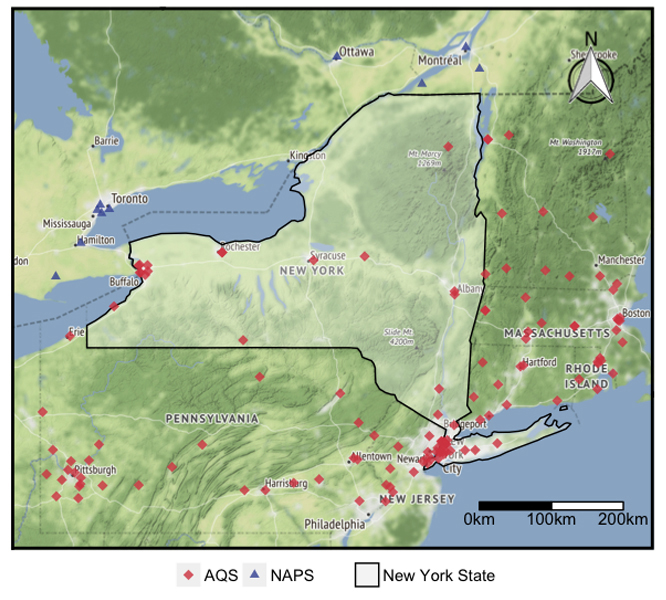
\includegraphics[width=0.55\textwidth]{img/ny.jpg}
        \label{fig:nys}
    \end{figure}
\end{frame}

\begin{frame}{Data and Methods}
    \begin{center}
        \textit{The Random Forest Algorithm}
    \end{center}
    \fbox{
    \begin{minipage}{0.4\textwidth}
        \textbf{AOD Gap-Filling Model}
        \begin{align*}
            &\mathrm{AOD_{\mathit{st}}}= \\
            &f(\mathbf{Snow/Cloud\;Params_{\mathit{st}},} \\
            &\mathrm{Meteorological_{\mathit{st}},} \\ 
            &\mathrm{Elevation_\mathit{s}, Spatial\;Coord_\mathit{s})}
        \end{align*}
    \end{minipage}
    }
    \fbox{
    \begin{minipage}{0.4\textwidth}
        \textbf{PM\tsub{2.5} Prediction Model}
        \begin{align*}
             &\mathrm{PM}\mathrm{_{2.5\mathit{st}}}=\\
             &f(\mathrm{\mathbf{Gapfilled\;AOD_{\mathit{st}}},PM_{2.5}\;Cov_{\mathit{st}},}\\
             &\mathrm{Meteorological_{\mathit{st}},}\\
             &\mathrm{Landuse_\mathit{s},Month_\mathit{t},Day_\mathit{t})}
        \end{align*}
    \end{minipage}
    }
    \begin{figure}
        \centering
        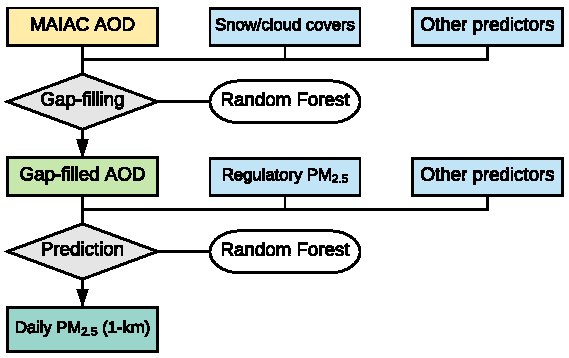
\includegraphics[width=0.47\textwidth]{img/steps.pdf}
    \end{figure}
\end{frame}

\begin{frame}{Results}
    \begin{center}
        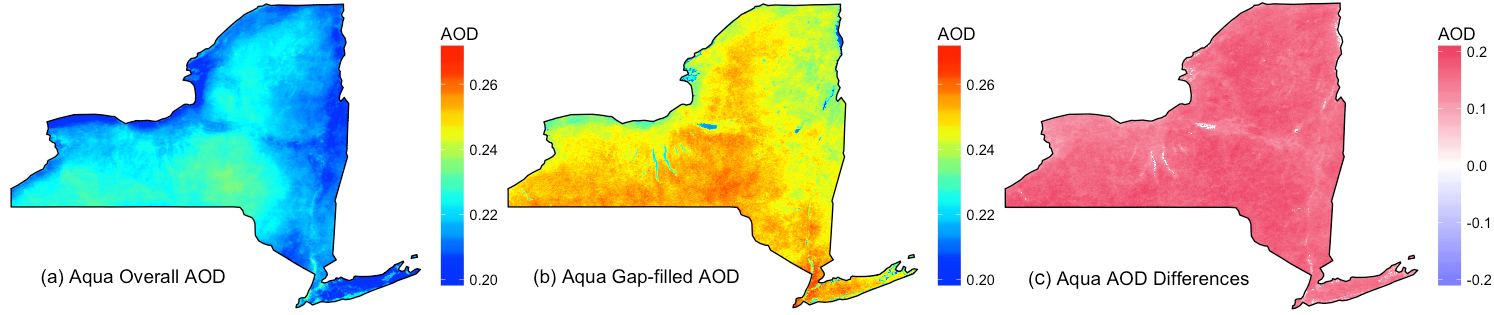
\includegraphics[width=\textwidth]{img/aod.jpg}
    \end{center}
    \begin{itemize}
        \item Generated AOD with a \textbf{100\%} coverage. The gap-filling model had a mean daily cross-validation R\tup{2} of 0.93
        \item The gap-filled AOD were significantly and constantly higher than the original AOD throughout the region (\textbf{hygroscopic growth of aerosol particles})
        \item At an annual level, AOD led to changes of PM\tsub{2.5} predictions by an absolute mean of $0.13\, \mu g/m^3$ and a maximum of $\sim 1\, \mu g/m^3$
    \end{itemize}
\end{frame}

\begin{frame}{Results (Cont'd)}
    \begin{center}
        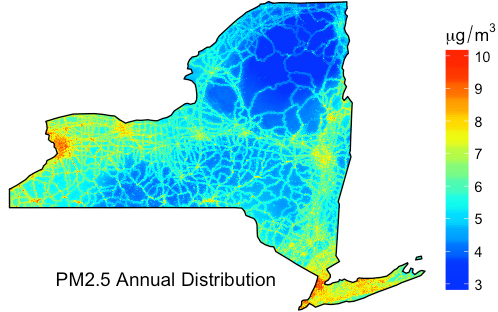
\includegraphics[width=0.6\textwidth]{img/pm25_nys.jpg}
    \end{center}
    \begin{itemize}
        \item Daily PM\tsub{2.5} predictions at a 1-km resolution
        \item Higher PM\tsub{2.5} levels were along with the roads and in the populated areas, which agreed with the PM\tsub{2.5} emission patterns in NYS (NEI 2014)
    \end{itemize}
\end{frame}

\begin{frame}{Summary}
    \begin{itemize}
    \item Fully-covered AOD data were produced by gap-filling with good model performance and reasonable distributions
    \item 1-km, daily PM\tsub{2.5} predictions derived from the gap-filled AOD were able to reflect detailed pollution patterns and small-scale terrain-driven features
    \item The methodology can be generalized to other areas with extensive cloud/snow cover (high latitude and altitude areas) to improve PM\tsub{2.5} exposure assessment
    \end{itemize}
    \vspace{1cm}
    \begin{spacing}{0.3}
    \scriptsize \textbf{Bi, J.}, Belle, J.H., Wang, Y., Lyapustin, A.I., Wildani, A., \& Liu, Y. (2019). Impacts of snow and cloud covers on satellite-derived PM\tsub{2.5} levels. \textit{Remote Sensing of Environment}, 221, 665–674. 
    \end{spacing}
\end{frame}